\documentclass[10pt,a4paper]{article}	
\usepackage{amsmath}
\usepackage{amsfonts}
\usepackage{amssymb}
\usepackage{cite}												% 支持引用多篇文献
\usepackage{CJK}													% 支持中文
\usepackage{indentfirst}                 						% 首行缩进宏包
\usepackage{graphicx}											% 支持图片的插入
\usepackage{subfigure}											% 支持插入子图
\usepackage[colorlinks,citecolor = blue, linkcolor=blue,hyperindex,CJKbookmarks]{hyperref}	% 链接功能
\usepackage{fancyhdr}											% 添加页眉

\graphicspath{{figs/}}                              				% 图片文件夹路径
\setlength{\parindent}{2em}										% 缩进距离为2个字符位置
\newcommand{\song}{\CJKfamily{song}}     						% 宋体
\newcommand{\hei}{\CJKfamily{hei}}       						% 黑体
\newcommand{\fs}{\CJKfamily{fang}}         						% 仿宋
\newcommand{\kai}{\CJKfamily{kai}}       						% 楷体
\newcommand{\li}{\CJKfamily{li}}         						% 隶书
\newcommand{\you}{\CJKfamily{you}}       						% 幼圆


\begin{document}

\begin{CJK*}{UTF8}{gkai}
%============================++题目和作者++================================
\title{贝叶斯网络学习笔记}					   							% 题目
\author{郝俊禹\thanks{Email:haojunyu2012@gmail.com}}				% 作者
%============================++++++++++++=================================
\date{}                                             				% 显示作者,不显示日期
\maketitle                                          				% 生成标题
\tableofcontents 												% 生成目录
\clearpage


\section{序}
鉴于这阶段所要研究的课题跟贝叶斯网络相关,所以就根据David Heckerman所写的技术报告《A Tutorial on Learning With Bayesian Networks》,在翻译的同时并结合自己对贝叶斯网络的理解写这个贝叶斯网络的学习心得,一方面是对自己理解的检验,也是当作一种记录。

%%date:			2014/06/09 20:40
%%position:		lab
%%author:		hjy
%%description:	
%%=====================================

\section{引言}
贝叶斯网络是一个图模型,能够将一系列变量之间的关系以图的形式表现出来。当它结合统计技术进行数据分析时有下列优点:
\begin{itemize}
\item 能体现各个变量的依赖关系,所以它能够处理部分数据缺失的情况。
\item 能够体现因果关系,因此能够加深对问题的理解并预测结果。
\item 模型既包含因果也包含概率语义,所以它是先验知识和数据的理想表示。
\item 贝叶斯统计方法\footnote{将关于未知参数的先验信息与样本信息综合,再根据贝叶斯公式,得出后验信息,最后根据后验信息去推断未知参数的方法} 结合贝叶斯网络能有效的避免数据的过拟合\marginpar{\textcolor{red}{\small 怎么就避免过拟合了?}}。
\end{itemize}





\section{人形机器人的相关概念及历史}
\subsection{人形机器人的定义及分类}
人形机器人,又称拟人机器人(humanoid),指是以模仿真人作为目的制造的机器人,大小上可以和真人差很远,也可以没有似人的外观,但有人的四肢和头等构造。\cite{1}

对于人形机器人的分类主要有以下几种\cite{2}:
\begin{description}
\item[拟人智能机器人(HIR)] 具有拟人智能的机器人,例如具有自行制定行为规划能力的机器人
\item[拟人情感机器人(HEmR)] 具有拟人情感的机器人,例如能与人进行情感交流的机器人
\item[拟人进化机器人(HEvR)] 具有自学习、自进化能力的机器人
\item[拟人行为机器人(HBR)] 例如步行机器人,舞蹈机器人,足球机器人等
\item[拟人形象机器人(HFR)] 具有拟人外观形象的机器人,例如虚拟电视节目主持人、电影演员、游戏角色
\item[拟人构造机器人(HAR)] 具有拟人内部构造的机器人,例如具有拟人内部器官组织构造,用于人体生理解剖,医学教学何研究的机器人
\end{description}


\subsubsection{Actroid-DER系列}
Actroid是一个与人非常类似的,由Osaka大学开发,KOKORO有限公司制造的人形机器人。外形如图\ref{fig:actroid}。\\
\begin{figure}[!htbp]
	\centering
	\caption{ACTROID}  
		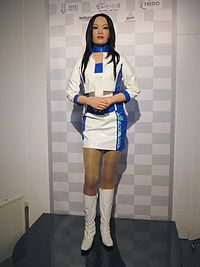
\includegraphics[scale=0.35]{figs/Actroid.jpg}
    	\label{fig:actroid}
\end{figure}



		
		
\bibliographystyle{unsrt}										% 按引用的先后顺序排列,比较次序为作者,年度和标题
\bibliography{mybib}												% 引用文件数据库在bib.bib文件中

\clearpage     
\end{CJK*}
\end{document}
